% Recuerda incluir en el preámbulo:
% \usetikzlibrary{babel}

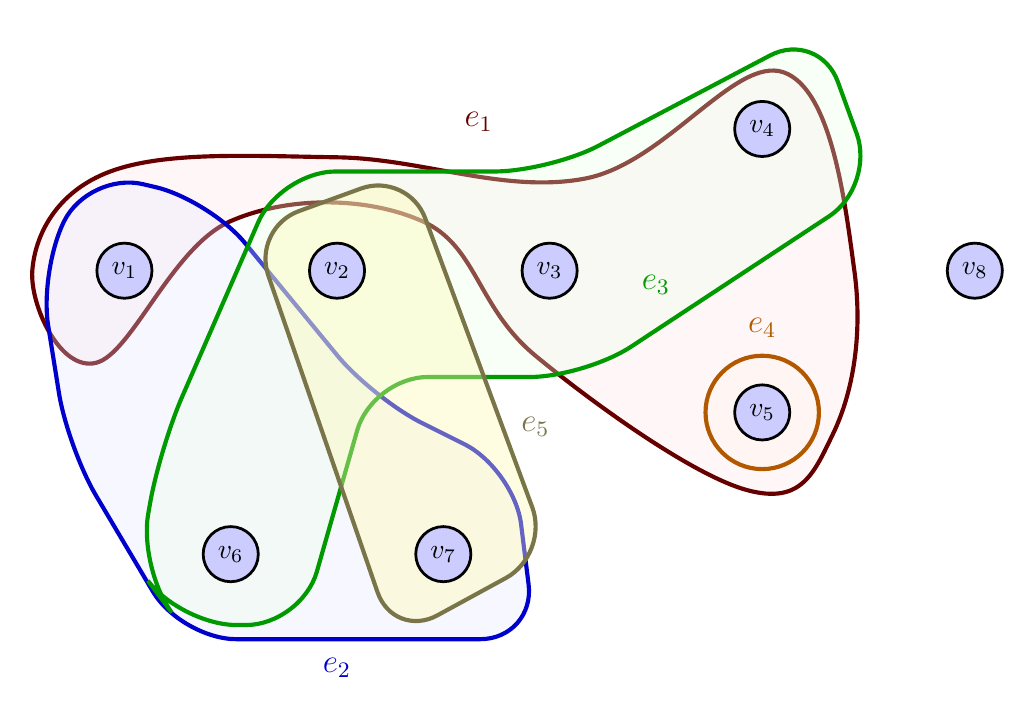
\begin{tikzpicture}[
  scale=0.9,
  every node/.style={circle, fill=blue!20, draw=black, line width=1pt, inner sep=2pt, minimum size=7mm}
]

  % ==========================================
  % 1. HIPERARISTAS (dibujadas al fondo)
  % ==========================================
  
  % e1 = {v1, v3, v4, v5} (Rojo oscuro - trazado orgánico y suave)
  \draw[red!40!black, line width=1.5pt, fill=red!10, fill opacity=0.3]
    plot [smooth cycle, tension=0.65] coordinates {
      (-1.3, 3.0)
      (-0.2, 4.4)
      (3.0, 4.6)
      (6.5, 4.3)
      (9.3, 5.8)
      (10.3, 3.0)
      (10.0, 0.7)
      (8.8, -0.1)
      (5.8, 1.8)
      (4.2, 3.7)
      (1.5, 3.7)
      (-0.4, 1.7)
    };
  \node[draw=none, fill=none, red!40!black, font=\large] at (5, 5.1) {$e_1$};

  % e2 = {v1, v6, v7} (Azul)
  \draw[blue!80!black, line width=1.5pt, fill=blue!10, fill opacity=0.3, rounded corners=20pt]
    (-1.2, 3) -- (-0.5, 4.4) -- (1.2, 4) -- (3.5, 1.2) -- (5.5, 0.2) -- 
    (5.8, -2.2) -- (0.8, -2.2) -- (-0.8, 0.5) -- cycle;
  \node[draw=none, fill=none, blue!80!black, font=\large] at (3, -2.6) {$e_2$};

  % e3 = {v2, v3, v4, v6} (Verde)
  \draw[green!60!black, line width=1.5pt, fill=green!10, fill opacity=0.3, rounded corners=20pt]
    (0.2, -1.2) -- (0.5, 0.5) -- (2.2, 4.4) -- (6, 4.4) -- (9.8, 6.4) -- 
    (10.6, 4.2) -- (6.5, 1.5) -- (3.5, 1.5) -- (2.5, -2) -- (0.8, -2) -- cycle;
  \node[draw=none, fill=none, green!60!black, font=\large] at (7.5, 2.8) {$e_3$};

  % e5 = {v2, v7} (Amarillo oscuro/Dorado)
  \draw[yellow!40!black, line width=1.5pt, fill=yellow!30, fill opacity=0.4, rounded corners=18pt]
    (1.8, 3.6) -- (4, 4.4) -- (6, -1) -- (3.8, -2.2) -- cycle;
  \node[draw=none, fill=none, yellow!40!black, font=\large] at (5.8, 0.8) {$e_5$};

  % e4 = {v5} (Naranja)
  \draw[orange!70!black, line width=1.5pt, fill=orange!10, fill opacity=0.3]
    (9,1) circle (8mm);
  \node[draw=none, fill=none, orange!70!black, font=\large] at (9, 2.2) {$e_4$};


  % ==========================================
  % 2. VÉRTICES (dibujados sobre las áreas)
  % ==========================================
  \node (v1) at (0,3) {$v_1$};
  \node (v2) at (3,3) {$v_2$};
  \node (v3) at (6,3) {$v_3$};
  \node (v4) at (9,5) {$v_4$};
  \node (v5) at (9,1) {$v_5$};
  \node (v6) at (1.5,-1) {$v_6$};
  \node (v7) at (4.5,-1) {$v_7$};
  \node (v8) at (12,3) {$v_8$};

\end{tikzpicture}
